\documentclass{aas}

\setsansfont[Extension = .ttf, BoldFont = *-Bold]{Euclid}

\begin{document}

\cntitle{《自动化学报》稿件加工样本%
  \thanks{收稿日期\
  XXXX-XX-XX \quad 录用日期\ XXXX-XX-XX}
  \thanks{Manuscript received Month Date, Year;
          accepted Month Date, Year}
  \thanks{国家重点基础研究发展计划 (973 计划) (XXXXX),
          国家高技术研究发展计划 (863 计划) (XXXXX),
          国家自然科学基金 (XXXXX) 资助}
  \thanks{Supported by National Basic Research Program of China
          (973 Program) (XXXXX),
          National High Technology Research and Development Program of China
          (863 Program) (XXXXX), and
          National Natural Science Foundation of China (XXXXX)}
  \thanks{本文责任编委\ XXX}
  \thanks{Recommended by Associate Editor BIAN Wei}
  \thanks{1. 中国科学院自动化研究所\ 北京\ 100190 \quad
          2. 中国科学院自动化研究所《自动化学报》编辑部\ 北京\ 100190}
  \thanks{1. Institute of Automation, Chinese Academy of Sciences,
          Beijing 100190\quad
          2. Editorial Office of \textsl{Acta Automatica Sinica},
          Institute of Automation, Chinese Academy of Sciences, Beijing 100190%
  }%
}
\cnauthor{尚书林\textsuperscript{1,\,2}\quad 左年明\textsuperscript{2}}

\cnabstract{摘要应涵盖全文. 摘要内容包括研究目的、方法、结果等, 注意不是标题的罗列, 能独立成文, 不能出现公式号和文献号. 英文摘要的书写, 请按英语习惯, 无文法及拼写错误, 用词准确.}

\cnkeyword{关键词 1; 关键词 2; 关键词 3; 关键词 4; 关键词 5}

\doi{10.16383/j.aas.cxxxxxx}
\cstr{32138.14.j.aas.cxxxxxx}

\entitle{Preparation of Papers for Acta Automatica Sinica}

\enauthor{SHANG Shu-Lin\textsuperscript{1,\,2}%
\qquad
ZUO Nian-Ming\textsuperscript{2}
}

\enabstract{An abstract should be a concise summary of the
significant items in the paper, including the results and
conclusions. Define all nonstandard symbols,
abbreviations and acronyms used in the abstract. Do not cite
references in the abstract.}

\enkeyword{keyword 1; keyword 2; keyword 3; keyword 4; keyword 5}

\cnaddress{尚书林, 左年明. 《自动化学报》稿件加工样本. 自动化学报, 202X,
\textbf{XX}(X): X$-$X}

\enaddress{Shang Shu-Lin, Zuo Nian-Ming.
Preparation of papers for Acta Automatica Sinica.
\textsl{Acta Automatica Sinica}, 202X, \textbf{XX}(X): X$-$X}

\maketitle

\pagestyle{aasheadings}


% \begin{multicols}{2}

%这一章为引言,无需写标题.

本文是《自动化学报》稿件 \LaTeX\ 模版的一个样例和使用说明.
模版的中文支持部分采用 \textsf{xeCJK}. 这一章为引言, 无需写标题 \cite{1}.


\section{准备稿件}

在正文开始之前, 需要%
\begin{itemize}
  \item 用~\verb|\cntitle|    来定义中文标题,
  \item 用~\verb|\cnauthor|   来定义中文作者,
  \item 用~\verb|\cnaddress|  来定义中文地址,
  \item 用~\verb|\email|      来定义 E-mail 地址,
  \item 用~\verb|\cnabstract| 来定义中文摘要,
  \item 用~\verb|\cnkeyword|  来定义中文关键词; 同样,
  \item 用~\verb|\entitle|    来定义中文标题,
  \item 用~\verb|\enauthor|   来定义英文作者,
  \item 用~\verb|\enaddress|  来定义英文地址,
  \item 用~\verb|\enabstract| 来定义英文摘要,
  \item 用~\verb|\enkeyword|  来定义英文关键词. 最后,
  \item 用~\verb|\maketitle|  来输出这些定义.
\end{itemize}

稿件首页应包括下列内容: 中英文标题、作者姓名、详细工作单位和邮政编码 (置于脚注位置)、摘要、关键词 ($3 \sim 8$ 个), 获基金资助的课题请在首页用中英文脚注说明, 基金项目英文名称请写全称而非缩写 (新投稿件请删除全部作者信息). 如该稿件不是原始性稿件 (如在某会议上发表过), 请作者务必在第一页用脚注注明.

\subsection{关于 \textbf{section} 标题的写法}

对于~\verb|section/subsection/subsubsection| 标题中的中文, 我们使用黑体; 当需要夹杂英文的时候, 英文使用粗体. 要生成当前 subsection 标题,可以这样写
\begin{verbatim}
\subsection{关于 \textbf{section} 标题的写法}
\end{verbatim}

\subsection{中文支持及中英文混排}

在您的 \LaTeX\ 系统已经安装了 \LaTeX\ 中文字体的情况下, 中文正文用宋体, 中文标题用黑体,
图片中的英文用 Euclid,英文标题用 EuclidBold. \% 用方正书宋, 希腊字符用 Euclid Symbol,
$\in$ 用 txsys 字体, $\ge$, $\le$ 用平的 Times New Roman.


当您编译 \path{.tex} 文件遇到类似以下的字体缺失警告时:
\begin{verbatim}
LaTeX Font Warning: Some font shapes were
not available, defaults substituted.
\end{verbatim}

请依次检查: 1) 您的 \LaTeX\ 系统是否已经安装了您使用的字体; 2) 字体的引用名称是否正确, 比如仿宋体的名称为 fangsong, 而不是 fs, 此时需要相应的修改 \path{aas.cls} 文件第 $64 \sim 69$ 行.

\subsection{\textbf{pdf}~的生成方法}

直接用~\verb|xelatex| 对 \path{.tex} 文件进行编译, 将自动生成 pdf 文件.
注意, 一般不要使用其他方法生成 pdf 文件.

\section{录用稿的格式及要求}

稿件要求论点明确, 论证充分, 语句通顺, 文字简练, 字迹工整.
% 定稿时论文和综述版面不超过7页; 短文不超过4页; 长论文版面可稍放宽. 凡版面超出过多、文字不流畅、编排混乱的稿件不给予发表.

\subsection{符号、计量单位和缩略词}

全文同一名词术语、人名、地名须前后一致. 每个字母、符号所表示的物理意义须前后一致, 并采用习惯表示法. 计量单位请采用国际单位制 (SI), 用规范符号表示, 如压力单位应用 $P$ (帕斯卡), 而不用``毫米汞注''. 文中中英文缩写词须在首次出现时注明全称. 文中统一使用英文逗号、句号, 英文表述部分逗号、句号后面加一个空格, 中文表述部分逗号、句号后面不必加空格.

\subsection{定理定义环境}

\begin{theorem}
定理测试
\end{theorem}

\begin{example}
例测试
\end{example}

\begin{definition}
定理测试
\end{definition}

\begin{corollary}
推论测试
\end{corollary}

\begin{lemma}
引理测试
\end{lemma}

\subsection{数学公式}


标准函数及常量用白正体;
普通变量用白斜体; 向量、矩阵用粗/白斜体均可;
5 个空间集合 $\mathbf{R}$、$\mathbf{C}$、$\mathbf{N}$、$\mathbf{Z}$、$\mathbf{Q}$
用粗正体,
其余集合用粗/白斜体 (以上均注意全文统一);
微分、积分、偏微分符号、数学期望、转置等排正体.
大写希腊字母如 $\Gamma\,\Delta\,\Theta\,\Lambda\,\Xi\,\Pi\,\Sigma\,
\Upsilon\,\Phi\,\Psi\,\Omega$ 排正体, 小写希腊字母排斜体. et al.,
etc., e.g., s.t. 排正体.

式 (1)、(2) 是两个简单单栏数学公式的例子.
\begin{equation}
Y_t^{e,k} = r^e\left( {{{\boldsymbol s}_t}} \right) + \gamma \max_{a^k} \left( {Q\left( {{{\boldsymbol s}_{t + 1}},{a^k};{{\boldsymbol \theta} ^k}} \right)} \right)
\end{equation}
\addtocounter{equation}{1}
\noindent
\parbox{\textwidth}{%
\medskip
\hrule
\medskip
\begin{equation}
  L^e\left( {{{\boldsymbol \theta} ^k}} \right)
= \mathrm{E}_{{\boldsymbol s}\sim\psi ,{\boldsymbol a}\sim\varphi ',\varphi '\sim{\pi ^*}\left( \psi  \right)}
  \left[ {\sum\limits_{k = 1}^N {{{\left( {Y_{}^{e,k} - {Q^k}\left( {{\boldsymbol s},a_{}^k;{{\boldsymbol \theta} ^k}} \right)} \right)}^2}} } \right]
\end{equation}
}

\newpage
\addtocounter{equation}{-2}
\begin{equation}
L({{{\boldsymbol \theta} ^k}}) = {P_s}{L^o}({{{\boldsymbol \theta} ^k}}) + ({1 - {P_s}}){L^e} ({{{\boldsymbol \theta} ^k}})
\end{equation}
\addtocounter{equation}{1}

式 (3) 是通栏公式的例子. 可以用环境~\verb|\end{|\linebreak\verb|multicols}|、
\verb|\begin{multicols}{2}| 以及~\verb|\oneco|\linebreak\verb|lumn| 产生.

\subsection{图表}

文中图、表只附最必要的, 标题需中英文对照.
图、表分别用阿拉伯数字全文连续编号,
图、表的引用一般需要遵循``先文后图/表''的原则.
\begin{enumerate}[label = {\makebox[\ccwd][l]{\arabic*)}}, labelsep = 0pt,
                  itemindent = 3\ccwd, leftmargin = 0pt]
  \item 字体: 图中标注文字英文用 Euclid 字体, 中文用宋体,
  消除锯齿的方法为平滑.
  \item 文中插图原图（以下 5 种格式均可: emf、PDF、Matlab 仿真图的 .fig 格式、Visio 的 .vsd 格式、Word 绘图的 .doc 格式图片）分别按顺序命名.
\end{enumerate}

注: 引用非开源图片时, 需要取得图片的著作权人的使用许可; 为提高文章的可读性, 请保留插图中出现的彩色线条和标志, 出版时网刊以彩图上传, 纸质刊则以黑白灰度图印刷.
以下是图的生成方式. 图 1 是一个双栏的图片示例,
图 2 是一个通栏的图片示例,
用~\verb|\end{multicols}|、\verb|\begin{multicols}{2}| 以及~\verb|\onecolumn| 环境.

\begin{figure}[htbp]
  \centering
  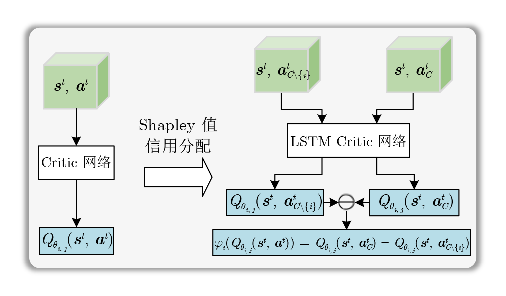
\includegraphics[width = \linewidth]{AAS-CN-2025-0624-3.eps}
  \bicaption{双栏图片示例}{An example graph in two column}
\end{figure}

《自动化学报》的表格采用的是三线表格式. 表 1 是一个通栏的表格示例, 表 2 是一个双栏的表格示例, 用~\verb|\end{multicols}|、\verb|\begin{multicols}{2}| 以及~\verb|\onecolumn| 环境.

\onecolumn

\begin{figure}[htbp]
    \centering
    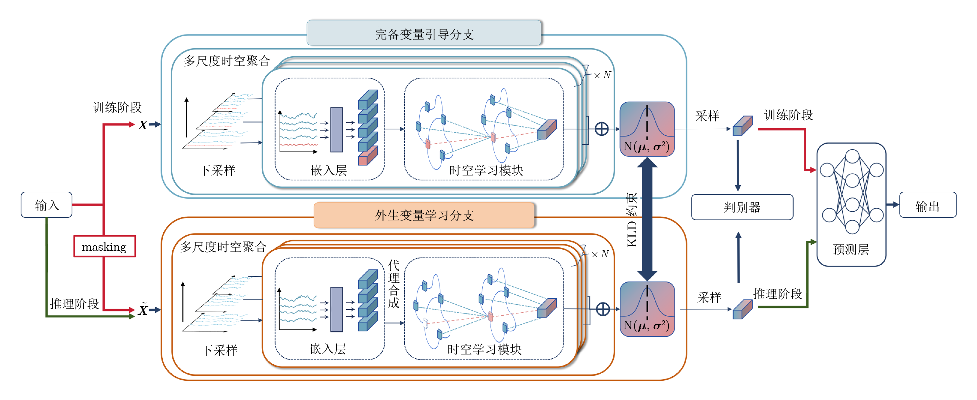
\includegraphics[width = \linewidth]{AAS-CN-2025-0653-2.eps}
    \bicaption{通栏图片示例}{An example graph in one column}
  \end{figure}

\begin{table}[htbp]
  \centering
  \renewcommand \arraystretch {1.2}
  \tabcolsep = 15pt\footnotesize
  \bicaption{通栏表格示例}{An example table in one column}
  \begin{tabular*}{\textwidth}{ccccc}
    \toprule
    对手~(OPP)                   & 比分~(CSU : OPP) & 团队决策所占比例 & 个体决策所占比例 & 团队决策与个体决策比值 \\
    \hline
    Cyberoos2001        & \phantom{0}3:0  & 71.5 & 28.5 & 2.51 \\
    FCPortugal2001      & \phantom{0}1:0  & 68.4 & 31.6 & 2.16 \\
    Gemini              & 26:0 & 59.7 & 40.3 & 1.48 \\
    Harmony             & \phantom{0}3:0  & 69.9 & 30.1 & 2.32 \\
    Lazarus             & 11:0 & 57.3 & 42.7 & 1.34 \\
    MRB                 & \phantom{0}2:0  & 63.2 & 32.8 & 1.93 \\
    SBCe                & \phantom{0}4:1  & 65.8 & 34.2 & 1.92 \\
    UvA\_Trilearn\_2001 & \phantom{0}1:0  & 54.9 & 44.1 & 1.24 \\
    UTUtd               & 10:0 & 70.7 & 29.3 & 2.41 \\
    WrightEagle2001     & \phantom{0}3:1  & 66.2 & 33.8 & 1.96 \\
    Average             &      & 64.8 & 35.2 & 1.84 \\
    \bottomrule
  \end{tabular*}
\end{table}

\begin{multicols*}{2}%开始双栏显示

\begin{table}[H]
  \centering
  \renewcommand \arraystretch {1.35}
  \footnotesize
  \bicaption{双栏表格示例}{An example table in two column}
  \begin{tabular*}{\linewidth}
    {>{\centering\arraybackslash}p{3\ccwd}
    *2{>{\centering\arraybackslash}p{\dimeval{.5\linewidth-1.5\ccwd-6pt}}}}
    \toprule
    序号 & BCDQN & PMDQN\\
    \hline
    1 & TP53 & TP53\\
    2 & FAM91A1 & PIK3CA\\
    3 & TNFRSF11B &TG\\
    4 & KCNQ3 & HHLA1\\
    5 & MYC & ASAP1\\
    6 & COL14A1 &CASC8\\
    7 & CCDC26 & SNORA12\\
    8 & CCN3 & MYC\\
    9 & PVT1 & PVT1\\
    10 & DSCC1 & RN7SL329\\
    \bottomrule
  \end{tabular*}
\end{table}

\subsection{参考文献}

参考文献只列公开出版的文献. 内部资料、未公开发行的论文集 (学位论文除外) 等不得作为文献引用, 必须引用时可放于出现页的脚注. 参考文献要按在文中出现的先后依次编号 $1,2, \cdots$, 即顺序编码制. 所引文献在正文中务请标注, 用 [ ] 表示. 作者人数超过六人用``et al.'', 否则请注明全部作者姓名. 注意文献条目中各项内容应该齐备, 否则将返回作者重新进行查证标引, 未被引用的文献不能列于参考文献列表中. 格式如本模板文末所示.

\LaTeX\ 的参考文献的引用比较方便, 比如我们想引用 Knuth 的 The \TeX book, 可以输入
``\verb|The|\linebreak
\verb|\TeX book\cite{1}|'' 得到想要的效果
``The\linebreak \TeX book\cite{1}''.
再比如我们输入``\verb|多模态优化问题|\linebreak\verb|\cite{2}|'' 得到想要的效果
``多模态优化问题\cite{2}''.

\subsection{作者简介注意事项}

文章末页需附作者中英文简介, 简介不超过 100 字, 包括作者姓名、职称、学习工作经历, 以及主要研究方向.


作者照片请选用清晰度较高的电子版证件照片.


\section{其他注意事项}

\begin{enumerate}[label = {\makebox[\ccwd][l]{\arabic*)}}, labelsep = 0pt,
                  itemindent = 3\ccwd, leftmargin = 0pt]
  \item 因本刊文章为国内外公开发表, 所有录用后稿件必须在本单位经保密审查.
  \item 请作者仔细地按照录用通知和该模版中的各项要求认真加工修改稿, 若修改稿不符合要求, 编辑部将退回作者重新修改直至合乎要求为止,  由此造成的稿件不能及时发表的责任由作者自负.
  \item 稿件经编辑加工和排版后, 编辑部将把 pdf 校样通过 E-mail 发送给全体作者, 请务必逐字逐句核对并返回校样. 除编辑和排版错误外请勿对校样内容作进一步的修改. 校样内容的修改将导致因需要请同行专家对稿件作进一步评议而延误文章发表, 因此而导致的后果和发生的费用将由作者承担.
  \item 在修改稿加工格式方面若有其他不明事宜, 请来函来电垂询. 感谢合作!
\end{enumerate}
\section{结论}

文章的结论请勿与摘要、前言等重复.

\subsection*{致谢}

文章作者可以在此处对支持和帮助其研究工作或本文写作的其他组织或人员表示感谢.
注意, 支持此研究的基金项目请直接标注在首页页脚处, 不用在此再次致谢.

\begin{thebibliography}{99}
\zihao{6} \addtolength{\itemsep}{0.2em} \urlstyle{rm}
  \bibitem{1} Wang X S, Gu Y , Cheng Y H, Liu A P, Chen C L P. Approximate policy-based accelerated deep reinforcement learning. {\sl IEEE Transactions on Neural Networks and Learning Systems}, 2020, \textbf{31}(6): 1820$-$1830

  \bibitem{2} Zhang C Q, Han Z B, Cui Y J, Hu Q. CPM-Nets: Cross partial multi-view networks. In: Proceedings of Advances in Neural Information Processing Systems (NIPS). Vancouver, BC, Canada: Curran Associates, 2019. 4077$-$4087
  \newcolumn
  \bibitem{3} Yan Hao, Wang Fu-Li, Sun Yu-Feng, He Da-Kuo. Abnormal condition identification based on Bayesian network parameter transfer learning for the electro-fused magnesia. \textsl{Acta Automatica Sinica}, 2021, \textbf{47}(1): 197$-$208\\
  (闫浩, 王福利, 孙钰沣, 何大阔. 基于贝叶斯网络参数迁移学习的电熔镁炉异常工况识别. 自动化学报, 2021, \textbf{47}(1): 197$-$208)

  \bibitem{4} Sun Y, Wang X G, Tang X O. Deep learning face representation from predicting 10 000 classes. In: Proceedings of the IEEE Conference on Computer Vision and Pattern Recognition (CVPR). Columbus, OH, USA: IEEE, 2014. 1891$-$1898

  \bibitem{5} Jin K H, McCann M T, Froustey E, Unser M. Deep convolutional neural network for inverse problems in imaging. \textsl{IEEE Transactions on Image Processing}, 2017, \textbf{26}(9): 4509$-$4522

  % \bibitem{6} Pang W Y, Fan J L, Jiang Y, LewisFrank L. Optimal output regulation of partially linear discrete-time systems using reinforcement learning. {\sl Acta Automatica Sinica}, 2021, {\bf 47}(x): 1$-$12 doi: 10.16383/j.aas.c190853, to be published \\
  % (庞文砚, 范家璐, 姜艺, LewisFrank L. 基于强化学习的部分线性离散时间系统的最优输出调节. 自动化学报, 2021, {\bf 47}(x): 1$-$12 doi: 10.16383/j.aas.c190853)

  % \bibitem{7} Shi W, Feng Y H, Cheng G Q, Huang H L, Huang J C, Liu Z, et al. Research on multi-aircraft cooperative air combat method based on deep reinforcement learning. {\sl Acta Automatica Sinica}, 2021, {\bf 47}(x): 1$-$14 doi: 10.16383/j.aas.c201059, to be published \\
  % (施伟, 冯旸赫, 程光权, 黄红蓝, 黄金才, 刘忠, 等. 基于深度强化学习的多机协同空战方法研究. 自动化学报, 2021, {\bf 47}(x): 1$-$14 doi: 10.16383/j.aas.c201059)

  \bibitem{8} Cheng Y H, Huang L Y, Wang X S. Authentic boundary proximal policy optimization. \textsl{IEEE Transactions on Cybernetics}, DOI: 10.1109/TCYB.2021.3051456

  \bibitem{9} Zhou B, Lapedriza A, Khosla A, Khosla A, Oliva A, Torralba A. Places: A 10 million image database for scene recognition. \textsl{IEEE Transactions on Pattern Analysis and Machine Intelligence}, 2018, \textbf{40}(6): 1452$-$1464
\end{thebibliography}

\begin{biography}[ssl.eps]
\noindent \textsf{尚书林}\quad
中国科学院自动化研究所博士研究生.
2002 年获得北京师范大学信息学院电子系学士学位.
主要研究方向为图像与视频压缩技术.\\
\mailto{aas\_editor@ia.ac.cn}

\noindent(\textbf{SHANG Shu-Lin}\quad
Ph.D. candidate at the
Institute of Automation, Chinese Academy of Sciences. He received
his bachelor degree from Beijing Normal University in 2002. His research
interests include image compression and video coding.)
\end{biography}

\begin{biography}[nmzuo.eps]
\noindent \textsf{左年明} \quad
中国科学院自动化研究所博士研究生.
2002 年获得山东大学数学学院学士学位.
主要研究方向为医学图像处理, CT 图像重建. 本文通信作者.\\
\mailto{aas\_editor@ia.ac.cn}

\noindent(\textbf{ZUO Nian-Ming}\quad
Ph.D. candidate at the Institute of Automation, Chinese Academy of Sciences. He received his bachelor degree from Shandong University in 2002. His research
interests include medical CT image reconstruction and medical image processing. Corresponding author of this paper.)
\end{biography}

\end{multicols*}

\end{document}
